\section{Thiết kế bản mẫu tương tác}

\subsection{Tổng quan bản mẫu}
Bản mẫu tương tác độ chi tiết cao (High-Fidelity Interactive Prototype) được xây dựng trên nền tảng Figma theo chuẩn kích thước điện thoại di động thông minh hiện đại ($430 \times 932\text{px}$, tương thích iPhone 14/15 Pro Max). Bản mẫu tái hiện đầy đủ và chân thực toàn bộ hành trình trải nghiệm người dùng với hệ thống màu sắc nhận diện thương hiệu chuẩn (Màu chủ đạo Xanh mòng két Teal \texttt{\#0D9488}, Màu cảnh báo Vàng hổ phách Amber \texttt{\#F59E0B}, Màu thành công Xanh ngọc lục bảo Emerald \texttt{\#10B981}), hệ thống kiểu chữ phân cấp rõ ràng và các tương tác chạm vuốt mượt mà.

\textit{Lưu ý về phạm vi}: Bản mẫu tương tác (Interactive Prototype) tập trung mô phỏng trọn vẹn các luồng hành vi giao diện người dùng (User Interface Flows) và logic phản hồi trạng thái phía máy khách; không đại diện cho một hệ thống cơ sở dữ liệu phân tán hay phần cứng xử lý backend hoàn chỉnh.

\subsection{Các màn hình bản mẫu}
Hệ thống bản mẫu bao gồm 4 nhóm màn hình tương tác chính tương ứng với 4 trụ cột nghiệp vụ cốt lõi:

\subsubsection{Luồng 1: Đặt lịch dịch vụ và Xác nhận tức thì}
Mô phỏng trải nghiệm chọn hồ sơ bé Poodle Bơ, chọn gói dịch vụ spa toàn diện, chọn khung giờ trống trong ma trận và nhận mã xác nhận lịch hẹn tức thì:

\begin{figure}[H]
\centering
\begin{minipage}[b]{0.31\textwidth}
    \centering
    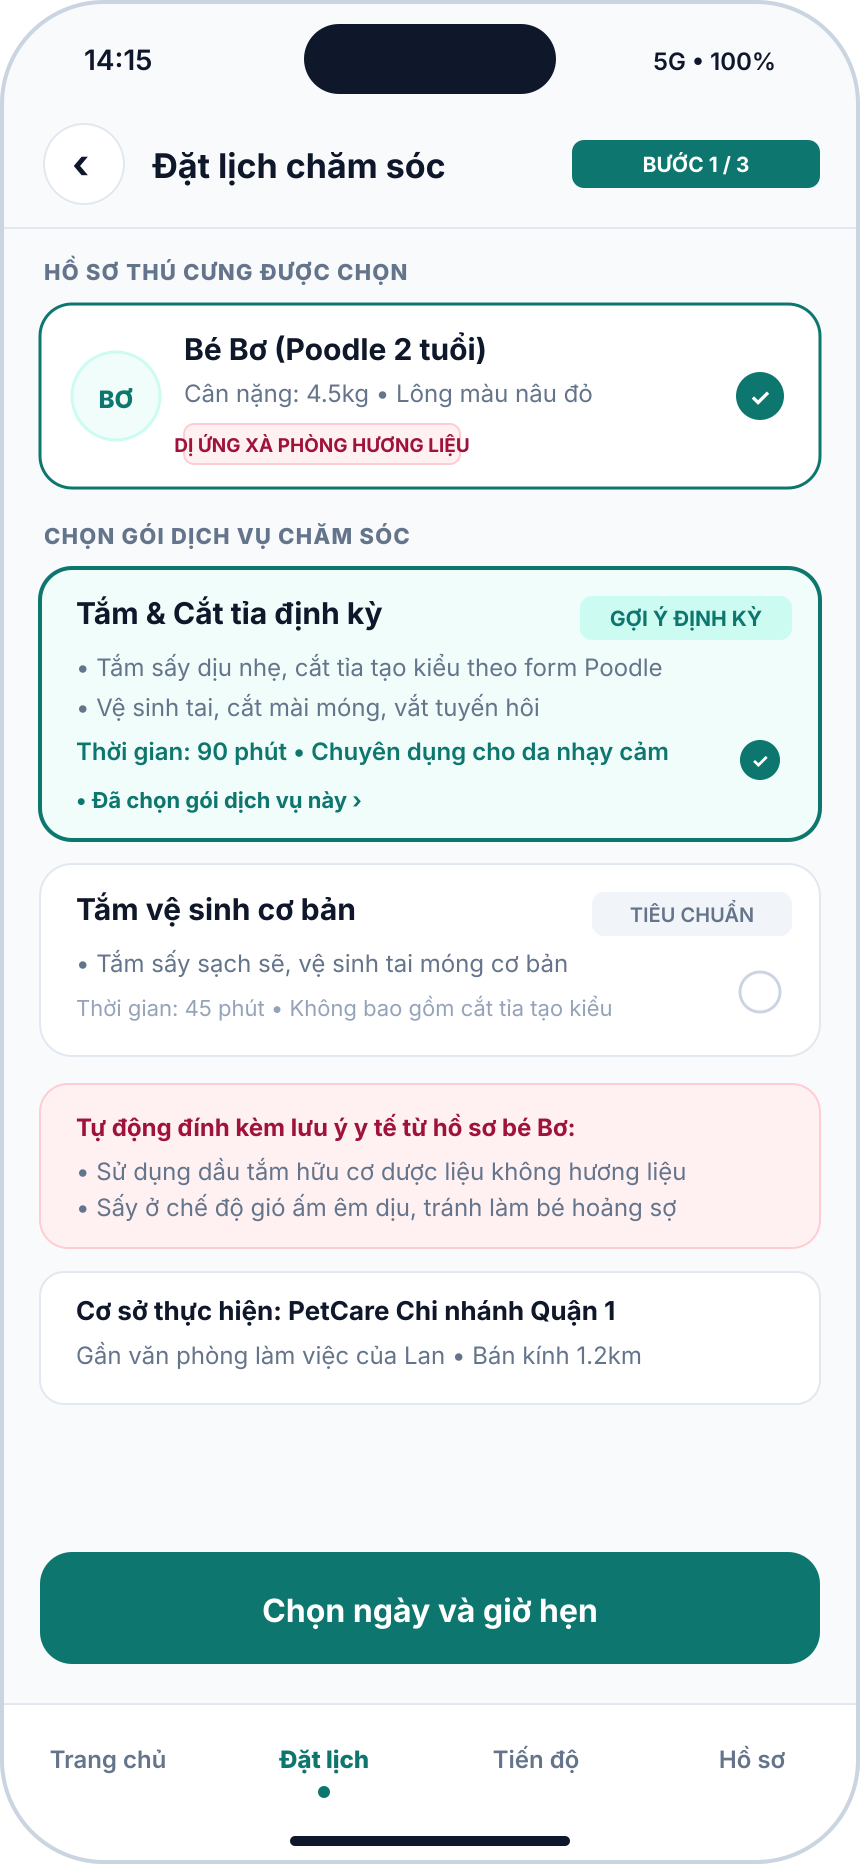
\includegraphics[width=\textwidth]{img/prototype/p1-g1/01_pet_service_selection.png}
    \caption*{(a) Chọn thú cưng \& Dịch vụ}
\end{minipage}\hfill
\begin{minipage}[b]{0.31\textwidth}
    \centering
    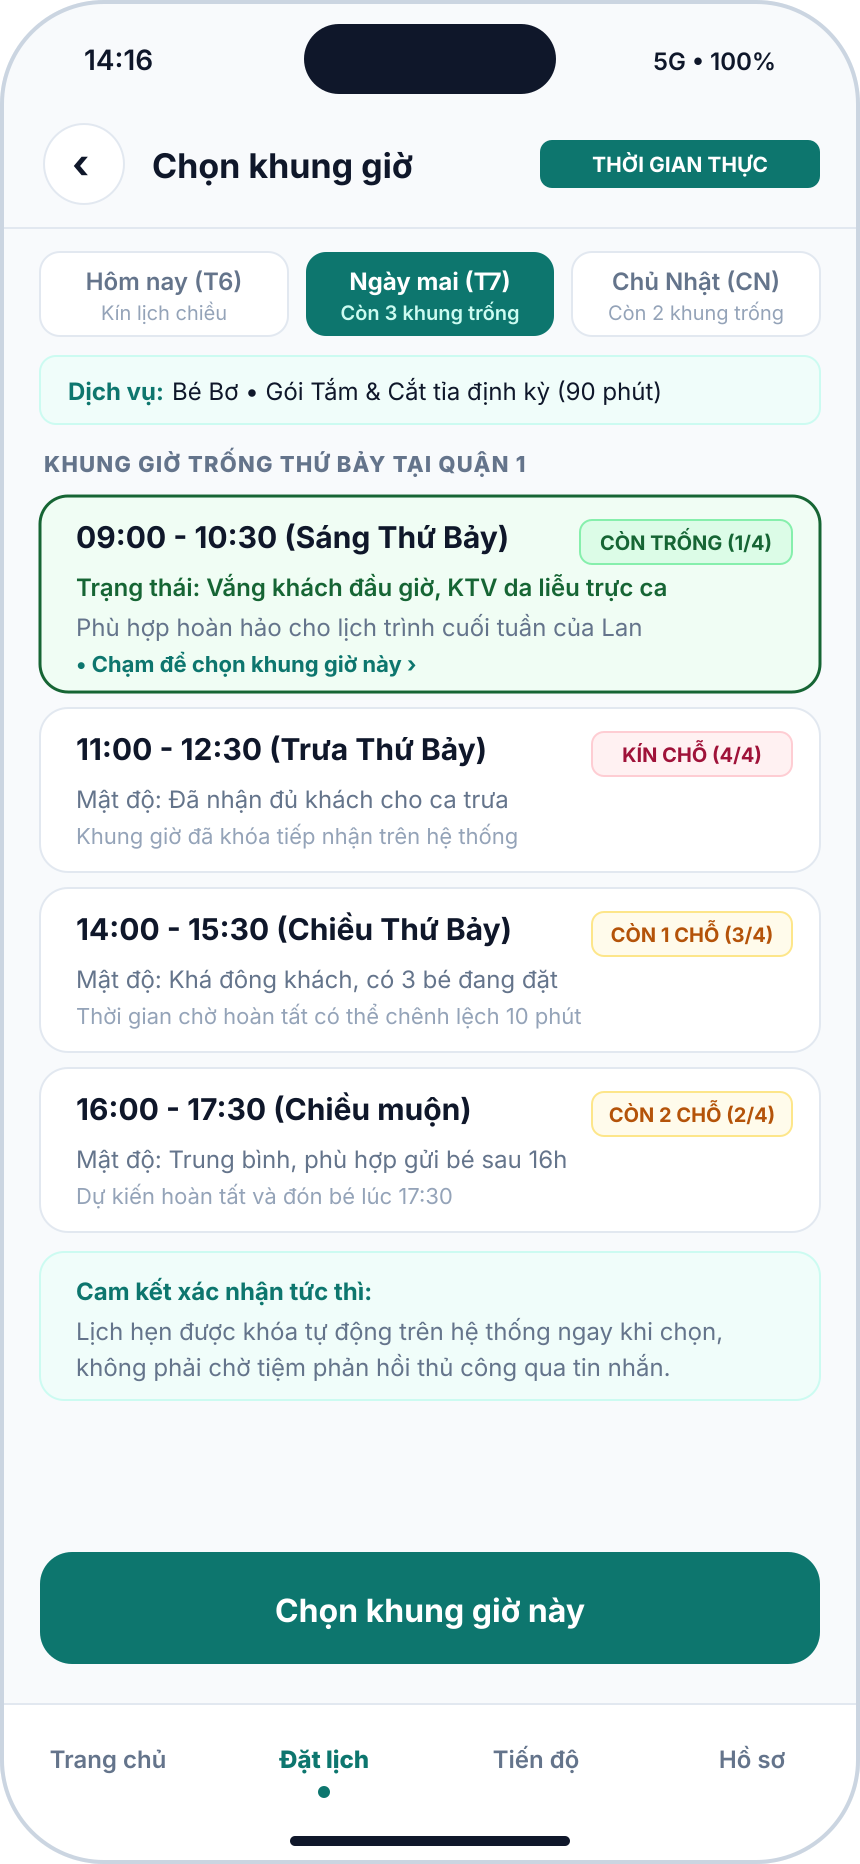
\includegraphics[width=\textwidth]{img/prototype/p1-g1/02_available_slots_matrix.png}
    \caption*{(b) Ma trận chọn giờ trống}
\end{minipage}\hfill
\begin{minipage}[b]{0.31\textwidth}
    \centering
    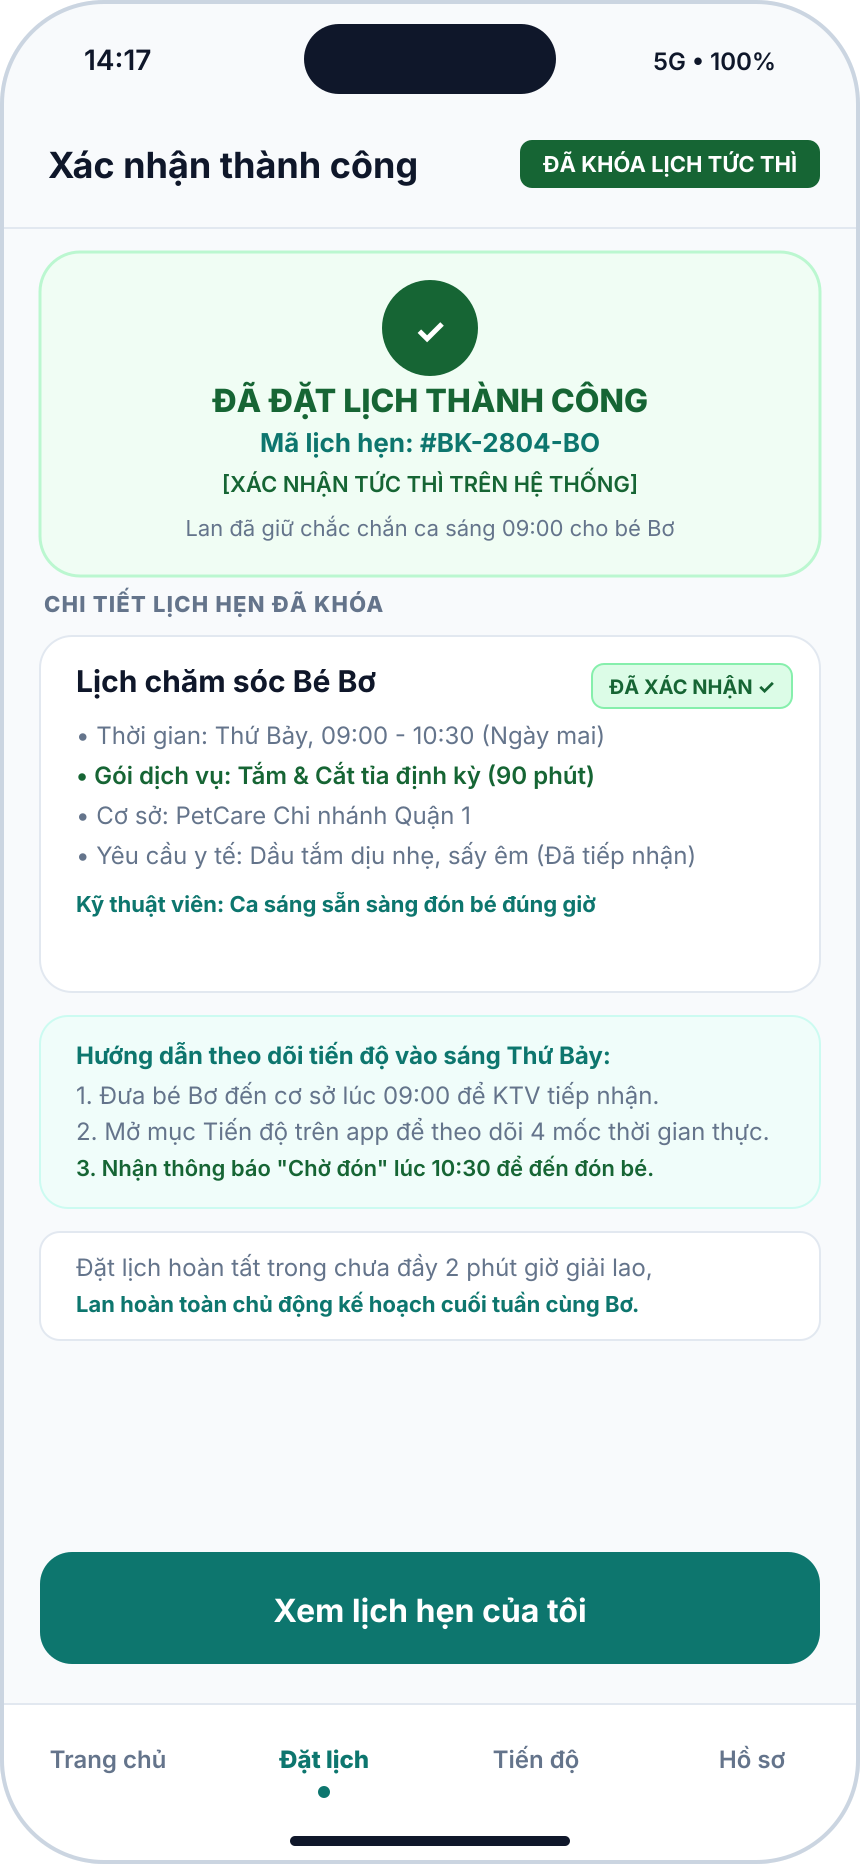
\includegraphics[width=\textwidth]{img/prototype/p1-g1/05_instant_booking_success.png}
    \caption*{(c) Xác nhận đặt lịch thành công}
\end{minipage}
\caption{Bản mẫu tương tác: Luồng đặt lịch dịch vụ và xác nhận tức thì}
\label{fig:proto_booking_flow}
\end{figure}

\subsubsection{Luồng 2: Bàn giao tiếp nhận và Khóa cam kết an toàn y tế}
Mô phỏng quá trình chủ nuôi quét mã QR tiếp nhận tại quầy, hệ thống tự động hiển thị Thẻ cảnh báo y tế (Amber Alert) về tiền sử viêm da dị ứng và nhân viên xác nhận cam kết quy trình an toàn:

\begin{figure}[H]
\centering
\begin{minipage}[b]{0.31\textwidth}
    \centering
    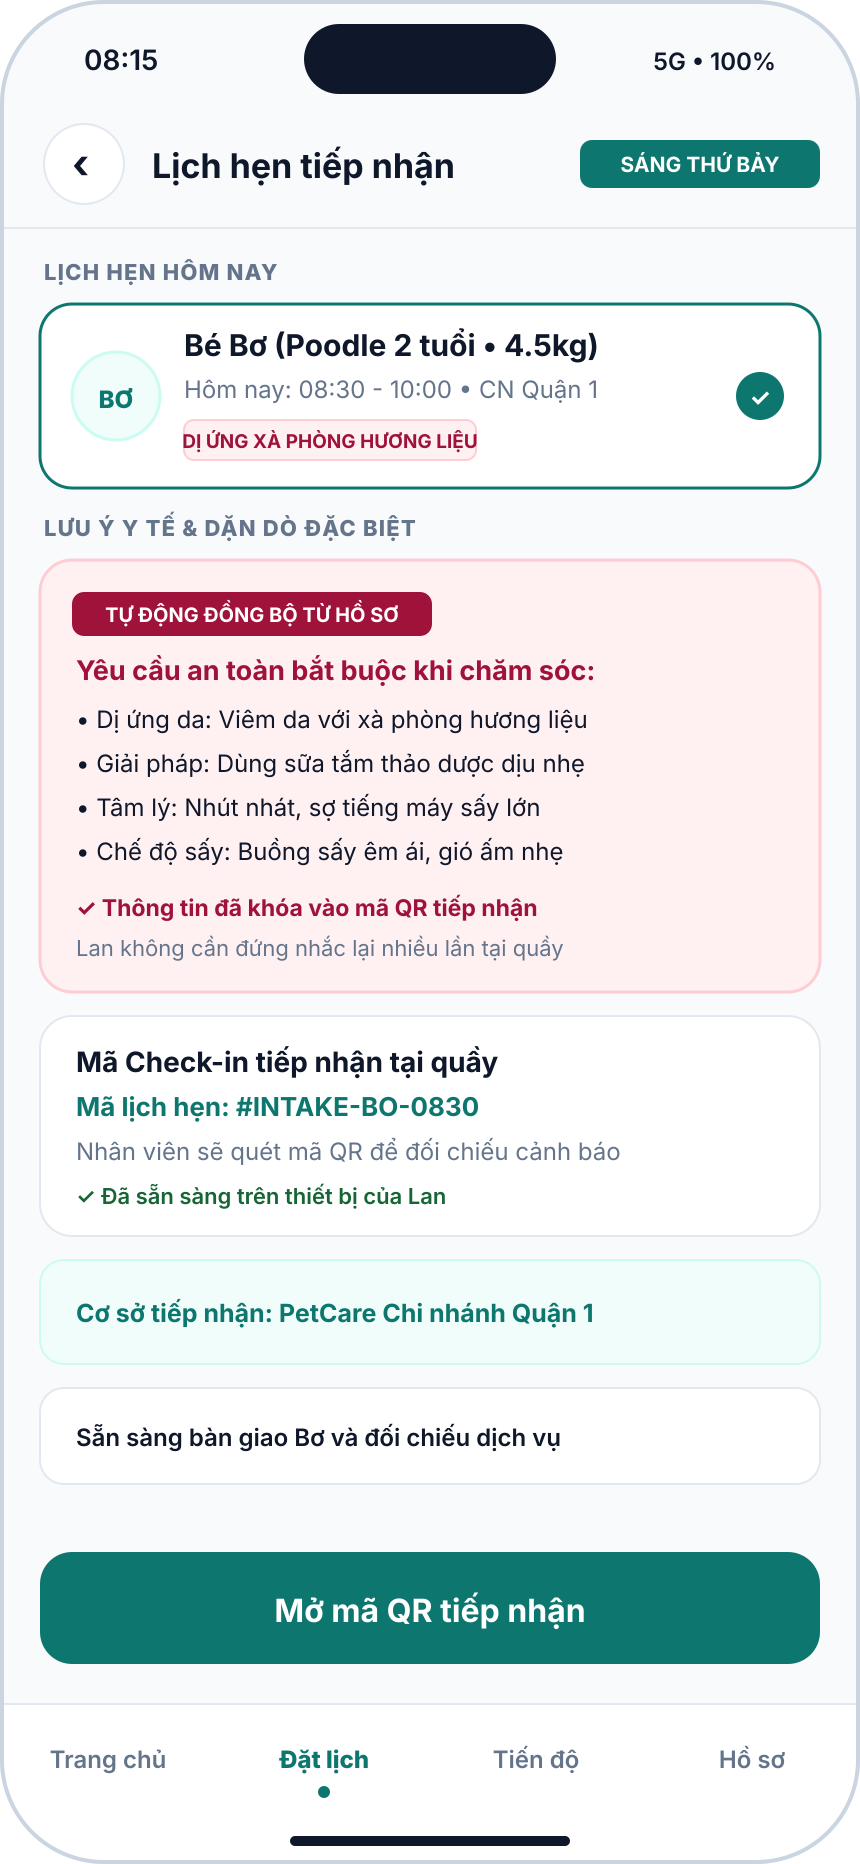
\includegraphics[width=\textwidth]{img/prototype/p1-g2/01_appointment_checkin_card.png}
    \caption*{(a) Thẻ tiếp nhận lịch hẹn}
\end{minipage}\hfill
\begin{minipage}[b]{0.31\textwidth}
    \centering
    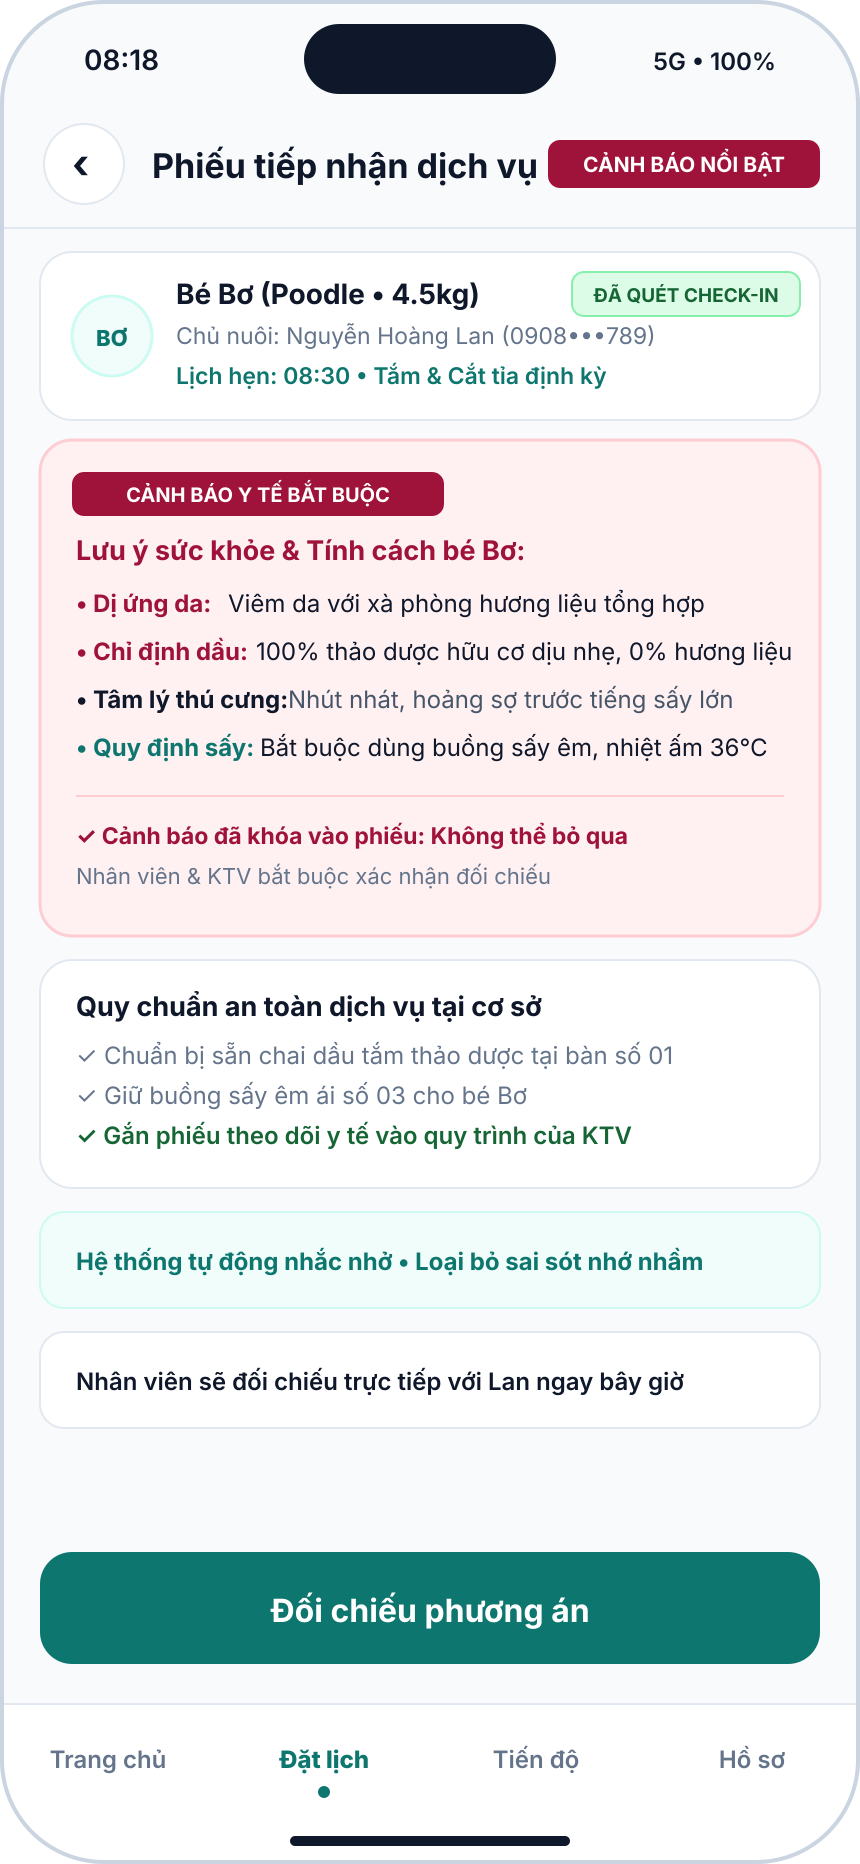
\includegraphics[width=\textwidth]{img/prototype/p1-g2/03_medical_alert_intake_view.png}
    \caption*{(b) Cảnh báo y tế dị ứng da}
\end{minipage}\hfill
\begin{minipage}[b]{0.31\textwidth}
    \centering
    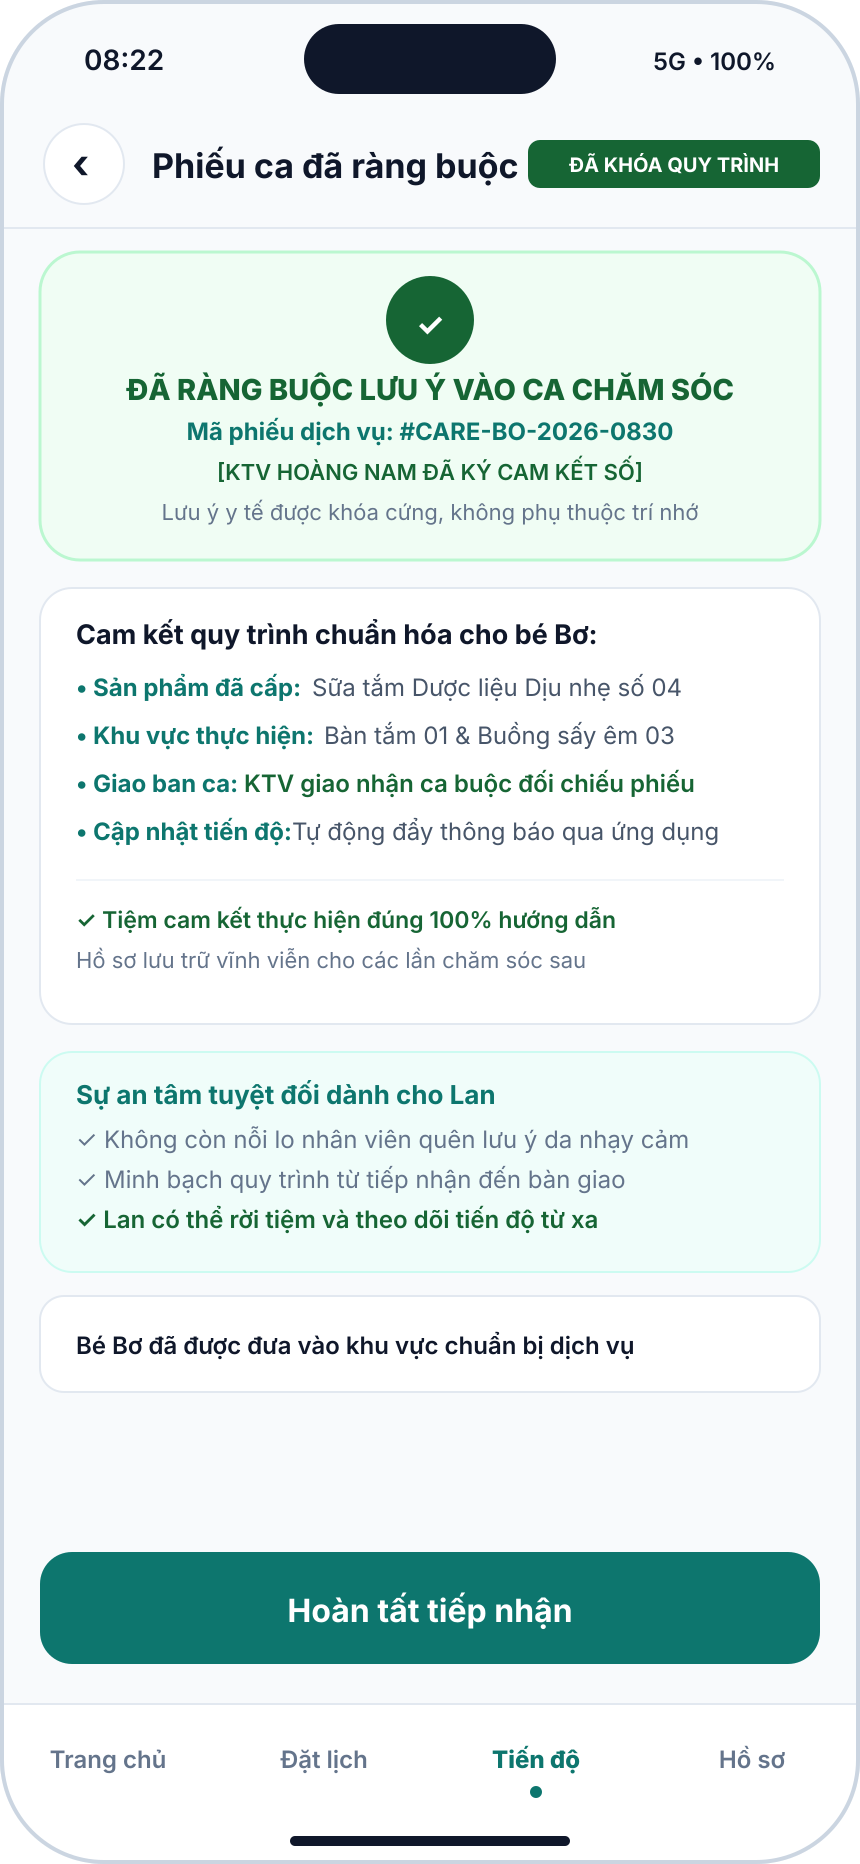
\includegraphics[width=\textwidth]{img/prototype/p1-g2/05_intake_safety_commitment_locked.png}
    \caption*{(c) Khóa cam kết an toàn}
\end{minipage}
\caption{Bản mẫu tương tác: Luồng tiếp nhận bàn giao và khóa dặn dò y tế}
\label{fig:proto_intake_flow}
\end{figure}

\subsubsection{Luồng 3: Theo dõi tiến độ theo thời gian thực (Live Tracking 4 mốc)}
Mô phỏng hành trình chăm sóc trực quan qua 4 mốc chuẩn kèm thông báo đẩy tự động khi chuyển mốc:

\begin{figure}[H]
\centering
\begin{minipage}[b]{0.31\textwidth}
    \centering
    
\includegraphics[width=\textwidth]{img/prototype/p1-g3/01_step1_received_status.png}
    \caption*{(a) Mốc 1: Đã tiếp nhận}
\end{minipage}\hfill
\begin{minipage}[b]{0.31\textwidth}
    \centering
    
\includegraphics[width=\textwidth]{img/prototype/p1-g3/02_step2_in_progress_care.png}
    \caption*{(b) Mốc 2: Đang chăm sóc}
\end{minipage}\hfill
\begin{minipage}[b]{0.31\textwidth}
    \centering
    
\includegraphics[width=\textwidth]{img/prototype/p1-g3/05_step4_ready_for_pickup.png}
    \caption*{(c) Mốc 4: Chờ đón thú cưng}
\end{minipage}
\caption{Bản mẫu tương tác: Luồng theo dõi tiến trình chăm sóc thời gian thực 4 mốc}
\label{fig:proto_tracking_flow}
\end{figure}

\subsubsection{Luồng 4: Tra cứu lịch sử chăm sóc và Quản lý hóa đơn}
Mô phỏng việc xem lại chi tiết gói dịch vụ, sản phẩm sữa tắm thảo dược đã sử dụng và hóa đơn điện tử:

\begin{figure}[H]
\centering
\begin{minipage}[b]{0.31\textwidth}
    \centering
    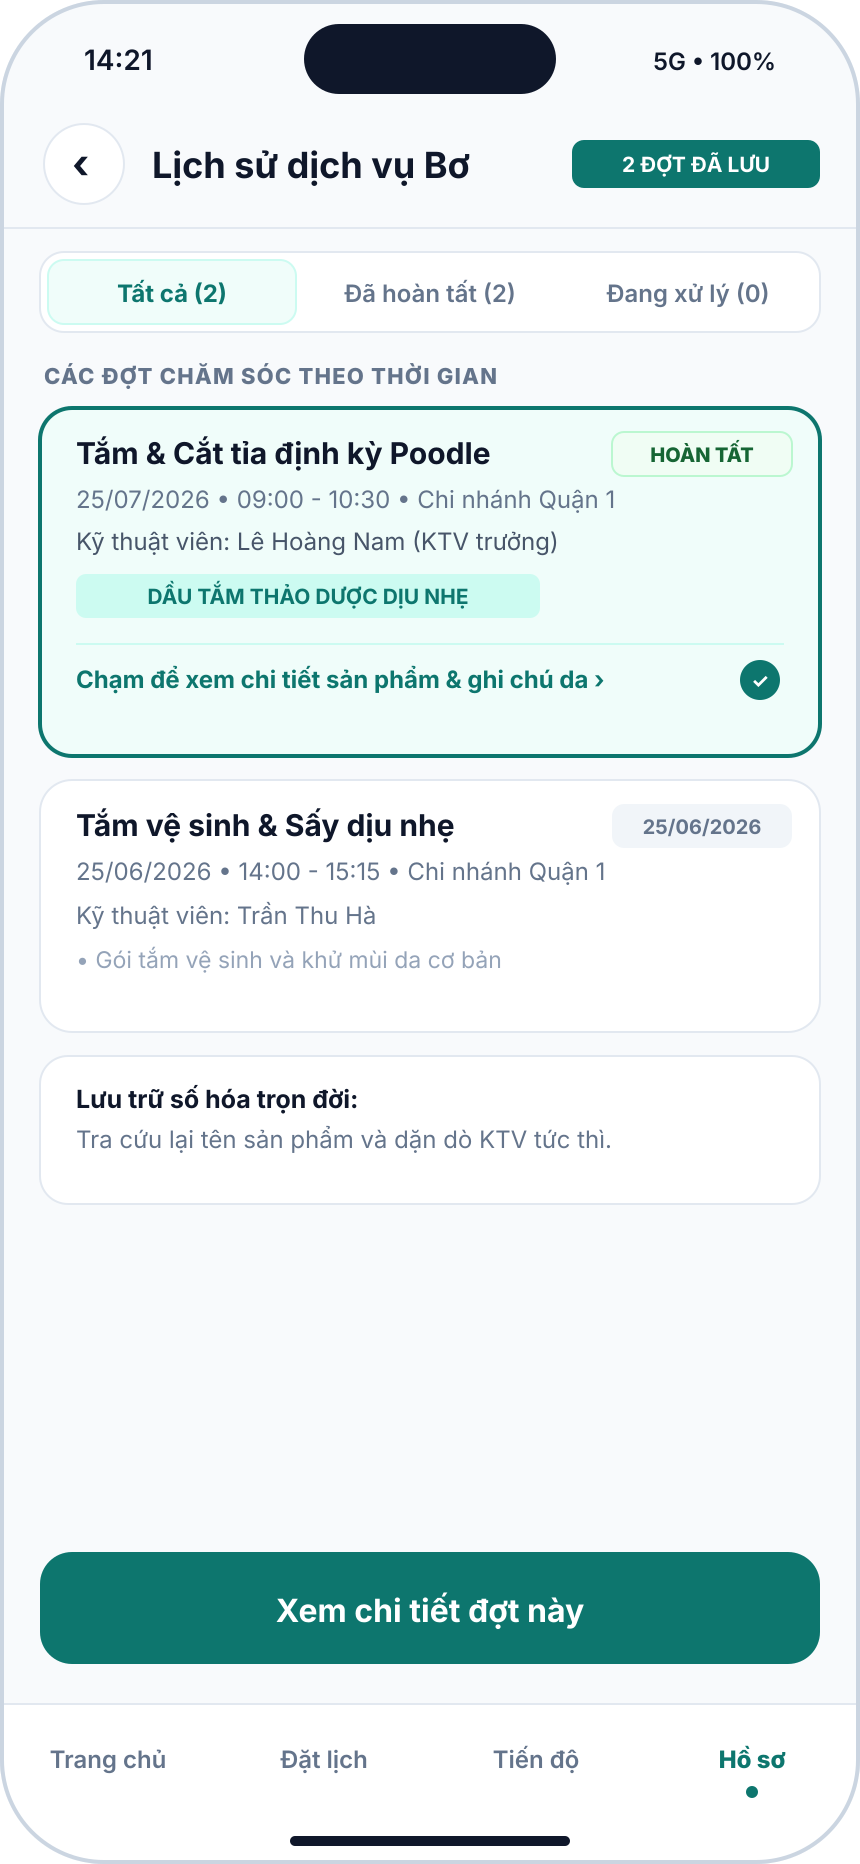
\includegraphics[width=\textwidth]{img/prototype/p1-g4/02_care_service_history_list.png}
    \caption*{(a) Danh sách lịch sử dịch vụ}
\end{minipage}\hfill
\begin{minipage}[b]{0.31\textwidth}
    \centering
    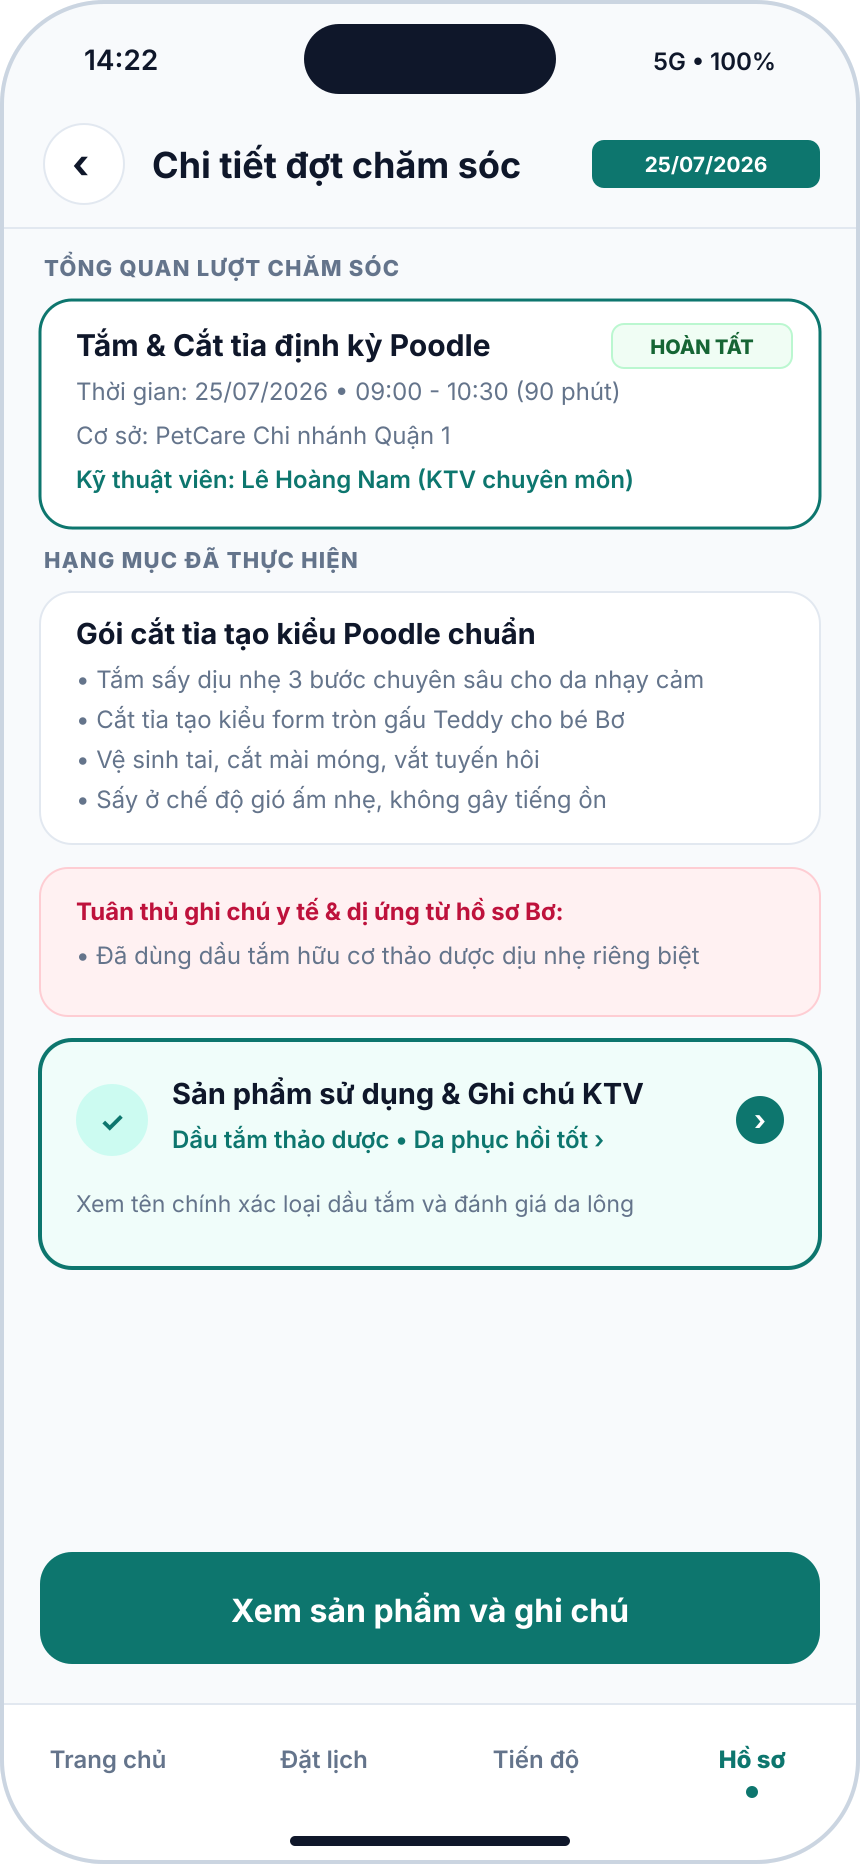
\includegraphics[width=\textwidth]{img/prototype/p1-g4/03_service_session_details.png}
    \caption*{(b) Chi tiết lượt chăm sóc}
\end{minipage}\hfill
\begin{minipage}[b]{0.31\textwidth}
    \centering
    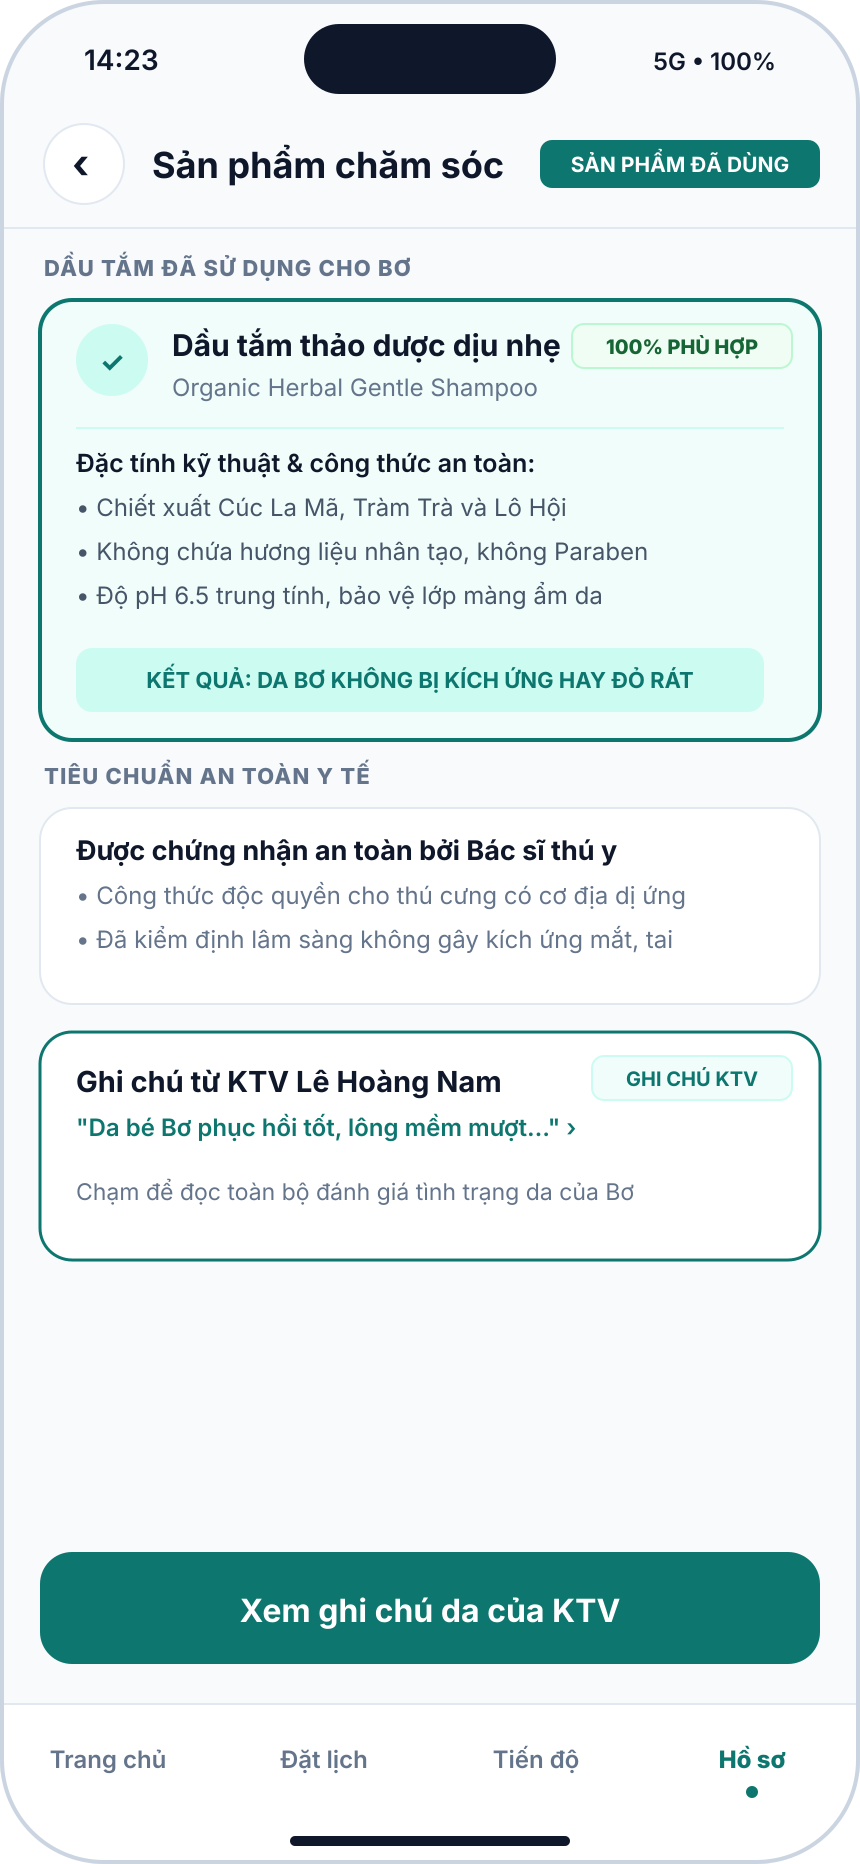
\includegraphics[width=\textwidth]{img/prototype/p1-g4/04_herbal_shampoo_product_verified.png}
    \caption*{(c) Xác nhận sữa tắm an toàn}
\end{minipage}
\caption{Bản mẫu tương tác: Luồng tra cứu lịch sử dịch vụ và chi tiết sản phẩm}
\label{fig:proto_history_flow}
\end{figure}

\subsection{Thiết kế tương tác}
Các tương tác then chốt (Key Interactions) được tối ưu hóa nhằm đảm bảo tính liền mạch và trực quan \cite{norman2013design}:
\begin{itemize}
    \item \textbf{Phản hồi trạng thái tức thì (Instant Feedback)}: Khi chọn một slot giờ trống, thẻ thời gian chuyển sang nền xanh đậm kèm hiệu ứng viền sáng và cập nhật tóm tắt chi phí ở chân trang ngay lập tức.
    \item \textbf{Cảnh báo chuyển động động (Active Pulsing Beacon)}: Tại mốc đang thực hiện trong Live Tracking, một vòng tròn ánh sáng chuyển động nhịp nhàng (Pulsing Animation) giúp người dùng nhận biết ngay tiến trình đang diễn ra mà không cần đọc lại toàn bộ chữ.
    \item \textbf{Hộp thoại xác nhận an toàn (Confirmation Modals)}: Các thao tác quan trọng (như hủy lịch hẹn, xác nhận hoàn tất bàn giao y tế) đều có modal xác nhận rõ ràng với các nút màu đối nghịch nhằm ngăn ngừa thao tác nhầm lẫn.
    \item \textbf{Xử lý trạng thái rỗng và lỗi (Empty \& Error States)}: Khi chưa có lịch hẹn hoặc khi mất kết nối mạng, màn hình hiển thị hình vẽ minh họa thân thiện kèm thông điệp hướng dẫn hành động khắc phục cụ thể.
\end{itemize}

\subsection{Lý giải thiết kế}
Mọi quyết định thiết kế trong bản mẫu đều được dẫn xuất chặt chẽ từ kết quả nghiên cứu và mục tiêu giải quyết điểm đau trong Proposal:
\begin{itemize}
    \item \textbf{Lý giải việc đưa Thẻ cảnh báo y tế vào ngay form đặt lịch}: Nghiên cứu cho thấy chủ nuôi rất sợ tiệm quên tiền sử dị ứng của thú cưng. Việc tự động đưa Thẻ Amber Alert nổi bật vào form giúp người dùng nhìn thấy ngay rằng hệ thống đã ghi nhớ dặn dò, mang lại sự an tâm tuyệt đối trước khi nhấn xác nhận.
    \item \textbf{Lý giải cấu trúc 4 mốc chuẩn trong Live Tracking}: 4 mốc (\textit{Đã nhận} $\rightarrow$ \textit{Đang chăm sóc} $\rightarrow$ \textit{Hoàn tất} $\rightarrow$ \textit{Chờ đón}) phản ánh chính xác chu trình tâm lý của chủ nuôi: từ lúc lo lắng chuyển giao, an tâm khi đang làm, nhẹ nhõm khi hoàn tất và chủ động sắp xếp thời gian di chuyển khi đến mốc chờ đón.
\end{itemize}
